%%%%%%%%%%%%%%%%%%%%%%%%%%%%%%%%%%%%%%%%%%%%%%%%%%%%%%%%%%%%%%%%%%%%%%%%%%
% 東京農工大学 工学部 機械システム工学科 中間発表前刷り用スタイルファイル
% Thanks to 佐久間先生 and 佐久間研の皆さん
% 書式設定部分のみ分離&いくつかコマンド定義&微修正 by 本堂
% 2013年度版でテンプレートに変更点があったので修正 by 恒岡
% 2016年度版でテンプレートに変更点があったので修正 by 熊谷
%%%%%%%%%%%%%%%%%%%%%%%%%%%%%%%%%%%%%%%%%%%%%%%%%%%%%%%%%%%%%%%%%%%%%%%%%%
\documentclass[a4paper,twocolumn,twoside,fleqn,leqno,10pt]{jarticle}
\usepackage[dvipdfmx]{graphicx}
\usepackage[dvipdfmx]{color}
\usepackage{bm}
\usepackage{fancyhdr}
%\usepackage{nidanfloat}
\usepackage{float}
%\date{\today 版}\西暦

\usepackage{booktabs}
\usepackage{amsmath}
\usepackage{amssymb}

%微分演算子関係
\newcommand{\dd}{\mathrm{d}} %微分演算子の"d"はローマン体
\newcommand{\diff}[2]{\frac{\mathrm{d}#1}{\mathrm{d}#2}} %常微分
\newcommand{\ddiff}[3]{\frac{\mathrm{d}^#1 #2}{\mathrm{d} #3^#1}} %高階常微分
\newcommand{\pdiff}[2]{\frac{\partial #1}{\partial #2}} %偏微分
\newcommand{\pddiff}[3]{\frac{\partial^#1 #2}{\partial #3^#1}} %高階偏微分

% 以下書式設定(一般) %%%%%%%%%%%%%%%%%%%%%%%%%%%%%%%%%%%%
\setlength{\hoffset}{-5mm}
\setlength{\voffset}{-9mm}
\setlength{\oddsidemargin}{0mm}
\setlength{\evensidemargin}{\oddsidemargin}
\setlength{\topmargin}{0mm}
\setlength{\headheight}{0mm}
\setlength{\headsep}{0mm}
\setlength{\textwidth}{180mm}
\setlength{\textheight}{255mm}
\setlength{\columnsep}{10mm}
\setlength{\topskip}{19.00pt}
\setlength{\mathindent}{4mm}
%\setlength{\kanjiskip}{0.00zw plus.1zw}
\setlength{\kanjiskip}{0.05zw plus.1zw}

\setlength{\floatsep}{3pt plus 1pt minus 1pt}
\setlength{\textfloatsep}{5pt plus 1pt minus 0.5pt}
\setlength{\intextsep}{5pt plus 1pt minus 0.5pt}
\setlength{\dblfloatsep}{3pt plus 1pt minus 1pt}
\setlength{\dbltextfloatsep}{3pt plus 1pt minus 1pt}

\setlength{\parskip}{0pt}
\setlength{\parindent}{1zw}
\setlength{\partopsep}{0pt}

% 英文概要設定 %
\def\abstract{\list{}{\listparindent=1zw \itemindent=\listparindent%
\leftmargin=5mm \rightmargin=\leftmargin}\item[]
\let\endabstract\endlist}

% 脚注の設定 %
\def\thefootnote{}

% 各節タイトル %
\def\thesection {\arabic{section}.}
\def\thesubsection {\arabic{section}$\,\cdot\,$\arabic{subsection}}
\def\thesubsubsection {\thesubsection$\,\cdot\,$\arabic{subsubsection}}

% 数式環境 %
\newdimen\vs % 機械学会書式(added by A.Sakuma)
\def\gyo[#1]{\\ \vbox to#1\vs\bgroup\vss}
\def\endgyo{\vss\egroup\vspace{-1.2mm}}%
\def\LABEL#1{\dotfill\hspace*{9.0mm}\label{#1}}
\def\LABELW#1{\dotfill\hspace*{23.0mm}\label{#1}}
\def\DOTFILL#1{\unitlength=1mm\begin{picture}(#1,3)
 \put(0,0){\makebox(#1,1.5)[b]{\dotfill}}\end{picture}}

% 図の配置設定 %
\def\topfraction{1.0} % 機械学会書式(changed by A.Sakuma)
\setcounter{bottomnumber}{6} % 機械学会書式(changed by A.Sakuma)
\def\bottomfraction{1.0} % 機械学会書式(changed by A.Sakuma)
\setcounter{totalnumber}{8} % 機械学会書式(changed by A.Sakuma)
\def\textfraction{0.0} % 機械学会書式(changed by A.Sakuma)
\def\floatpagefraction{0.7} % 機械学会書式(changed by A.Sakuma)
\setcounter{dbltopnumber}{8}% 機械学会書式(changed by A.Sakuma)
\def\dbltopfraction{1.0} % 機械学会書式(changed by A.Sakuma)
\def\dblfloatpagefraction{0.7} % 機械学会書式(changed by A.Sakuma)
% ```````````````````````````````````````````````````````
% 以下書式設定(特殊) %%%%%%%%%%%%%%%%%%%%%%%%%%%%%%%%%%%%
\makeatletter
% 各節タイトル %
\def\section{\@startsection {section}{1}{0.0ex}{1.62ex}{1.62ex}{\center\rm\bf}}%%セクションを太字に2018諸岡
\def\subsection{\@startsection{subsection}{2}{0.0ex}{1.0ex}{.5ex}{\rm}}%タイトルの後改行
%タイトルを中央揃えにする場合は@startsectionの第6引数を{\center\bf}にする
\def\subsubsection{\@startsection{subsubsection}{3}
{3.0ex}{0.0ex}{-6.0ex}{\rm}}
\def\quote{\list{}{\rightmargin=10mm \leftmargin=\rightmargin}\item[]}%
\long\def\@makecaption#1#2{
\vskip 10pt 
\setbox\@tempboxa\hbox{#1  #2}
\ifdim \wd\@tempboxa >\hsize \settowidth{\labelwidth}{#1} \textwidth=\hsize
\addtolength{\textwidth}{-\labelwidth}\addtolength{\textwidth}{-6pt}
\tabcolsep=2pt\begin{tabular*}{\hsize}{@{\extracolsep{\fill}}lp{\textwidth}}
 #1&\setlength{\baselineskip}{9.0pt}\setlength{\lineskip}{-0.5pt}#2\\
 \end{tabular*}\par\else\hbox to\hsize{\hfil\box\@tempboxa\hfil} \fi}
\def\fnum@figure{\small{Fig.\thefigure}}

% 引用の設定 %
\def\@cite#1#2{$^{\hbox{\scriptsize({#1\if@tempswa , #2\fi})}}$}
\def\thebibliography#1{\section*{{\bf{文  献}}\@mkboth
 {REFERENCES}{REFERENCES}}\list
% {(\hfill\arabic{enumi}\hfill)}{\settowidth\labelwidth{1pt} \leftmargin 30pt
 {(\hfill\arabic{enumi}\hfill)}{\settowidth\labelwidth{1pt} \leftmargin\labelwidth %文献のインデントを左端にした。
 \advance\leftmargin\labelsep
 \usecounter{enumi}}
 \def\newblock{\hskip .11em plus .33em minus .07em}
 \sloppy\clubpenalty4000\widowpenalty4000
 \sfcode`\.=1000\relax}

% 数式環境 %
\def\@eqnnum{\hbox to .01pt{}
 \rlap{\rm \hskip -0.125\displaywidth(\theequation)}}
\def\eqnarray{\stepcounter{equation}\def\@currentlabel{\p@equation\theequation}%
 \global\@eqnswtrue\m@th\global\@eqcnt\z@\tabskip\@centering\let\\\@eqncr
 $$\everycr{}\halign to\displaywidth\bgroup\hskip\@centering$\displaystyle
 \tabskip\z@skip{##}$\@eqnsel&\global\@eqcnt\@ne \hfil$\displaystyle{{}##{}}$\hfil
 &\global\@eqcnt\tw@ $\displaystyle{##}$\hfil\tabskip\@centering
 &\global\@eqcnt\thr@@ \hb@xt@\z@\bgroup\hss##\egroup\tabskip\z@skip\cr}  
\def\@eqnnum{\hbox to .01pt{}%
 \rlap{\rm \hskip -0.10\displaywidth(\theequation)}}
\def\fnum@table{Table \thetable.}
\def\thetable{\@arabic\c@table}

%% Figure 環境中で Table 環境の見出しを表示・カウンタの操作に必
\newcommand{\figcaption}[1]{\def\@captype{figure}\caption{#1}}
\newcommand{\tblcaption}[1]{\def\@captype{table}\caption{#1}}

\makeatother


\usepackage{ifthen}
\newcommand{\secret}[2]{
  \ifthenelse{\equal{#1}{m}}{
    \thispagestyle{fancy}
    \lhead{
      \vspace{-10mm}
      \begin{picture}(0,0)
        \fboxrule=0.5mm
        \hspace{#2}\fcolorbox{red}{white}{{\large {\bf \textcolor{red}{専攻外秘}}}}
    \end{picture}
    }
  }{
    \thispagestyle{fancy}
    \lhead{
      \vspace{-10mm}
      \begin{picture}(0,0)
        \fboxrule=0.5mm
        \hspace{#2}\fcolorbox{red}{white}{{\large {\bf \textcolor{red}{学科外秘}}}}
      \end{picture}
    }
  }
}
\newcommand{\pagenum}[1]{%
\chead{}
\rhead{ \sf{#1} }%%フォントを変更2018諸岡
\lfoot{}
% \cfoot{ \bf{#1} } %ページ数
\cfoot{}
\rfoot{}
}
\renewcommand{\headrulewidth}{0pt}
\renewcommand{\footrulewidth}{0pt}

\pagestyle{empty}
\renewcommand{\title}[2]{
%\twocolumn[%
 \begin{center}
 {\Large\bf #1}\\%日本語タイトルも太字に変更2018諸岡
 {\bf #2}%英語タイトル太字に変更
\end{center}
\vspace{-5mm}
}
\renewcommand{\author}[3]{
 \begin{flushright}
  % \begin{center}
  \begin{small}
    #1\hspace{6mm}#2\hspace{3mm}#3\\
  \end{small}
  % \end{center}
 \end{flushright}
% ]
}
\newcommand{\keyword}[1]{
 \begin{center}{\small
  \begin{tabular*}{150mm}{lp{140mm}}
    \hspace{-17mm}\sl{Key Words} %%Key Word(細字イタリック)に変更2018諸岡
    \rm{: #1}
  \end{tabular*}
 }\end{center}
\vspace{-3mm}
}

%% \newcommand{\keyword}[1]{
%%  \begin{center}{\small
%%   \begin{tabular*}{150mm}{lp{140mm}}
%%   \hspace{-17mm}$\sl{KeyWord}$: &%%Key Word(細字イタリック)に変更2018諸岡
%% #1
%%   \end{tabular*}
%%  }\end{center}
%% \vspace{-3mm}
%% }

%\newenvironment{doctmp}{\begin{document}}{\end{document}}
%\renewenvironment{document}{\begin{doctmp}\begin{small}}{\end{small}\end{doctmp}}
% キーワード
% \begin{center}{\small
 % \begin{tabular*}{138mm}{lp{112mm}}
 % $\mathit{Key Words}$: &
%Upright Posture Control Probrems,
%Agonist, Antagonist, 
%Bio-Motion Controll Problems,
%Muscle, 
%Biological soft tissue 
%Viscoelasticity, 
%2-DOF Robot, 
%  \end{tabular*}
 %}\end{center}
%\vspace{-3mm}
%\setlength{\baselineskip}{4.38mm}    %%% 60行指定(機械科前刷仕様)
%\setlength{\baselineskip}{4.30mm}
%\setlength{\baselineskip}{4.65mm}
\setlength{\vs}{\baselineskip}
\vspace{-\baselineskip}
%\begin{small}
\setlength{\baselineskip}{4.30mm}
%%%%%%%%%%%%%%%%%%%%%%%%%%%%%%%%%%%%%%%%%%%%%%%%%%%%%%%%%%%%%%%%%%%%%%%%%%%%%%

\usepackage{jtygm}
\usepackage{ikuo}
\pagenum{1-9}%ページ番号
\secret{m}{0mm}                 %学外秘/専攻外秘の設定.学部はb(学外秘),修士はm(専攻外秘)にする.
                                %第2引数は位置の調整用.-側に大きくすれば左に寄る.+側に大きくすれば右に寄る.
\newcommand{\FIGDIR}{./fig}	%図を置くディレクトリを指定する
				%Makefileとは連動していないので注意
\begin{document}
\twocolumn[%
\title{ほげ症候群の予防を目的としたほげワクチンの開発}{Development of Hoge Vaccine for Prevention of Hoge Syndrome}
\author{本堂 貴敏}{水内研究室}{Takatoshi HONDO}

\begin{abstract}
ココにはアブストを書こう.
\end{abstract}
\keyword{Hoge, Huga, Hage}
]
\begin{small}
\section{緒  言}
ほげ症候群が近年大きな社会問題となっている\cite{Ikuo:doctor}.
ほげ症候群の蔓延により,ソフトウェア生産性の低下や
プログラミング初心者の混乱などの悪影響が多数報告されている.
ほげ症候群が重大な精神疾患であり,かつ社会に多大なる
悪影響を与えているにも関わらず,これまでほげ症候群に関する
対策は全く行われてこなかった.本研究では,ほげ症候群を予防するための
ワクチンの開発を目的とする.本研究では特にほげの原理に基づいた
ワクチン開発を試みる.
\section{ほげ症候群の主な症例}
ほげ症候群とは主に以下のような症状全般を指す\cite{Hondo:hohoge2006}.
\begin{itemize}
\item 気がつくと指が勝手に``hoge''と打っている.
\item ``hogan''と打とうとすると指が勝手に``hogen''と動く.
\item 気がつくと「ほげー」っとしている.
\item 気がつくとほげだけで会話が成立している.
\end{itemize}
\section{ほげの公式の導出}
\subsection{ほげの原理}
ほげの原理は次式で与えられる\cite{Kawamura:hogege2010}.
\begin{eqnarray}
\int_{-\infty}^\infty \mathrm{hoge}(x,y) dx = \left( \pdiff{\mathrm{hoge}}{y} \label{hoge} \right)_{x = 0}
\end{eqnarray}
ただし$\mathrm{hoge}(x,y)$はほげ母関数である.
\subsection{ほげの公式}
式(\ref{hoge})から以下の式が自明である.
\begin{eqnarray}
1 + 1 = 2
\end{eqnarray}
本研究では上式をほげの公式と呼ぶ.
\section{ほげワクチンの実験}
前章での議論より以下の反応でほげ症候群が予防できると考えられる.
\begin{eqnarray}
\mathrm{Hoge^{2+} \ + 2e^{-} \ \rightarrow \ Hoge}
\end{eqnarray}
ワクチン生成装置のスペックをTable \ref{spec}に示す.
\begin{table}[b]
\caption{Motor parameters}
\label{spec}
\begin{center}
\begin{tabular}{c c}
\toprule
$R$ & $11.2\,\mathrm{\Omega}$ \\
$L$ & $4.52 \times 10^{-4}\,\mathrm{H}$ \\
$J_\mathrm{m}$ & $1.29 \times 10^{-7}\,\mathrm{kg \cdot m^2}$ \\
$K_\mathrm{m\phi}\,(=K_\mathrm{b})$ & $1.62 \times 10^{-2}\,\mathrm{N \cdot m / A}$ \\
$F_\mathrm{m}$ & $2.28 \times 10^{-7}\,\mathrm{N \cdot m \cdot s / rad}$ \\
$E$ & $24\,\mathrm{V}$ \\
$\gamma$ & 84 \\
\bottomrule
\end{tabular}
\end{center}
\end{table}
実験結果を\figref{piyo}に示す.また、被験者がほげた結果を\figref{hogeta}に示す。

\begin{figure}[b]
\begin{center}
\framebox{ほげは世界を救う}
\caption{Result of experiment}
\figlabel{piyo}
\end{center}
\end{figure}

\begin{figure}[b]
\begin{center}
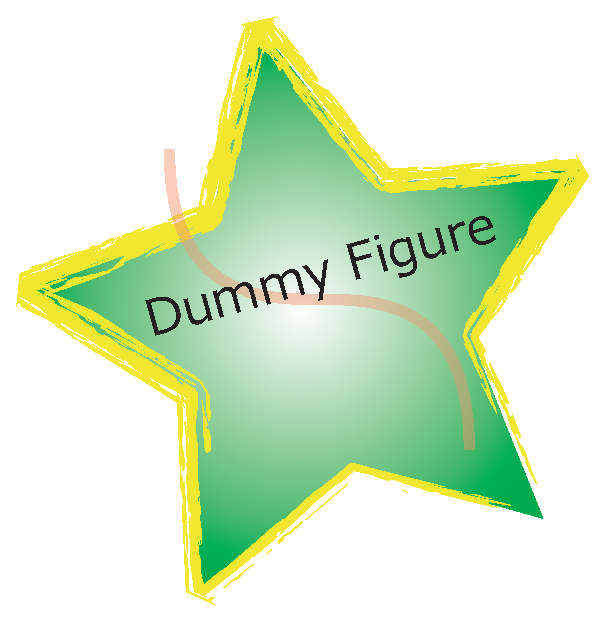
\includegraphics[width=0.75\hsize]{\FIGDIR/fig1.eps}%
\caption{Result of hogeta}
\figlabel{hogeta}
\end{center}
\end{figure}
\section{結  言}
ほげワクチンの開発は不可能である.
そのため、ほげ症候群にならないように予防をする必要があると考えられる。


%% \begin{thebibliography}{99}
%% \small
%%  \setlength{\kanjiskip}{0.0zw plus.01zw} %
%%  \setlength{\baselineskip}{9pt}        %
%%  \setlength{\itemsep}{0.2pt}             %
%%  \setlength{\lineskip}{0pt}              %
%%  \setlength{\normallineskip}{0.2pt}      %


%% \bibitem{hogege} 川村マサキ,
%% ほげの可能性と適用限界に関する実験的研究,日本ほげ学会ほげ工学部門講演会,(2010).

%% \bibitem{hoooge} 日本ほげ医学会編,
%% 本当は怖いほげの医学,(2011),捕鯨出版.

%% \bibitem{hohoge} 本堂貴敏,
%% ほげの力学,(2006),pp.11-43,ほげ出版.

{
\small
 \setlength{\kanjiskip}{0.0zw plus.01zw} %
 \setlength{\baselineskip}{9pt}        %
 \setlength{\itemsep}{0.2pt}             %
 \setlength{\lineskip}{0pt}              %
%% \scriptsize %%←どうしても入らない時は,このコメントをはずすと少し小さくなる.
\bibliographystyle{junsrt}
\bibliography{reference}
}



%% \end{thebibliography}
\end{small}
\end{document}
